%% ****** Start of file apstemplate.tex ****** %
%%
%%
%%   This file is part of the APS files in the REVTeX 4 distribution.
%%   Version 4.1r of REVTeX, August 2010
%%
%%
%%   Copyright (c) 2001, 2009, 2010 The American Physical Society.
%%
%%   See the REVTeX 4 README file for restrictions and more information.
%%
%
% This is a template for producing manuscripts for use with REVTEX 4.0
% Copy this file to another name and then work on that file.
% That way, you always have this original template file to use.
%
% Group addresses by affiliation; use superscriptaddress for long
% author lists, or if there are many overlapping affiliations.
% For Phys. Rev. appearance, change preprint to twocolumn.
% Choose pra, prb, prc, prd, pre, prl, prstab, prstper, or rmp for journal
%  Add 'draft' option to mark overfull boxes with black boxes
%  Add 'showpacs' option to make PACS codes appear
%  Add 'showkeys' option to make keywords appear
% \documentclass[aps,prl,preprint,groupedaddress]{revtex4-1}
%\documentclass[aps,prl,preprint,superscriptaddress]{revtex4-1}
%\documentclass[aps,prl,reprint,groupedaddress]{revtex4-1}

\documentclass[%
 reprint,
%superscriptaddress,
%groupedaddress,
%unsortedaddress,
%runinaddress,
%frontmatterverbose,
%preprint,
%showpacs,preprintnumbers,
%nofootinbib,
%nobibnotes,
%bibnotes,
 amsmath,amssymb,
 aps,
%pra,
%prb,
prl
%rmp,
%prstab,
%prstper,
%floatfix,
]{revtex4-1}


\usepackage{epsfig}
\usepackage{natbib}
\usepackage{subfig}
\usepackage[]{graphicx}
\usepackage{rotating}
\usepackage{here}
\usepackage{calc}
\usepackage{multirow}
\usepackage{amsfonts}
\usepackage{amssymb}
\usepackage{color}
\usepackage{nomencl}
\usepackage{textcomp}
\usepackage{eurosym}
\usepackage[ansinew]{inputenc}
\usepackage[bookmarks=true,bookmarksnumbered=true]{hyperref}

\graphicspath{{figures/EPS/}}


% You should use BibTeX and apsrev.bst for references
% Choosing a journal automatically selects the correct APS
% BibTeX style file (bst file), so only uncomment the line
% below if necessary.
%\bibliographystyle{apsrev4-1}

\begin{document}

% Use the \preprint command to place your local institutional report
% number in the upper righthand corner of the title page in preprint mode.
% Multiple \preprint commands are allowed.
% Use the 'preprintnumbers' class option to override journal defaults
% to display numbers if necessary
%\preprint{}

%Title of paper
\title{Linear Stability Analysis of a submerged cylinder.}

% repeat the \author .. \affiliation  etc. as needed
% \email, \thanks, \homepage, \altaffiliation all apply to the current
% author. Explanatory text should go in the []'s, actual e-mail
% address or url should go in the {}'s for \email and \homepage.
% Please use the appropriate macro foreach each type of information

% \affiliation command applies to all authors since the last
% \affiliation command. The \affiliation command should follow the
% other information
% \affiliation can be followed by \email, \homepage, \thanks as well.
\author{Leo M. Gonz\'alez, Esteban Ferrer}
\affiliation{%
  Technical University of Madrid (UPM)\\
  Arco de la Victoria 4, 28040 Madrid, Spain
}%

\author{Juan M. Gimenez}
\affiliation{
Centro de Investigaci\'on de M\'etodos Computacionales (CIMEC) - UNL/CONICET \\
Facultad de Ingenier�a y Ciencias H�dricas - Universidad Nacional del Litoral \\
Paraje El Pozo, Santa Fe, Argentina
}%
%\affiliation{
% Facultad de Ingenier\'ia y Ciencias H\'idricas\\
% Universidad Nacional del Litoral, Santa Fe, Argentina
%}

\date{\today}% It is always \today, today,
             %  but any date may be explicitly specified

\begin{abstract}
This Letter describes how the results of a global stability analysis of a classical circular cylinder are affected when the cylinder is submerged in a two phase gravitational flow. The flow behavior is governed by both the Reynolds and Froude numbers, while the depth of the cylinder has been varied to create different scenarios for the stability analysis. The baseflow obtained by the Navier-Stokes equations has been analyzed, and the Hopf bifurcation has been obtained for a fixed Froude number. The critical Reynolds number and the frequency of the most unstable mode have been compared to the classical solution without free surface and gravity effects. The most unstable mode is deformed and distorted according to the free surface location, while the critical frequency and the critical Reynolds numbers are both affected by the gravity and the free surface presence.
\end{abstract}

% insert suggested PACS numbers in braces on next line
\pacs{}
% insert suggested keywords - APS authors don't need to do this
%\keywords{}

%\maketitle must follow title, authors, abstract, \pacs, and \keywords
\maketitle

%=====================================================================================
\section{Introduction}
\label{S:Intro}
%=====================================================================================

The interaction between the viscous wake of a submerged object and the free surface position is a problem that deserves attention. Several reasons sustain its importance, \cite{Dimas89} justifies the study due to its potential relevance for the remote sensing of the ocean surface from satellites, while \cite{Reichl05,Bouscasse14} outline its application to the design of offshore structures and vessels.
It is well known that in the absence of free surface and gravity, the von Karman vortex street generated by flow past an infinitely long circular cylinder produces a two dimensional time periodic flow for Reynolds numbers between approximately 47 and 189 \cite{JacksonJFM87,ProvansalJFM87,WilliamsonPoF88,miller1994control}. This work focuses on the changes produced in the stability of this flow when the cylinder is submerged and a free surface separating two different fluids in the presence of gravity. Different steady baseflows have been studied and a linear global stability analysis has been performed in order to quantify the differences when free surface and gravity are added to the problem. Previous authors performed stability analysis of idealized problems such as simple vortex structures \cite{ohring1991interaction,fontane2008stability} and analytic shear flows \cite{Dimas89}. To the authors knowledge, this constitutes the first study where a global stability analysis is performed on a Navier-Stokes computed solution in the presence of high discontinuities in density caused by the free surface. In order to gain insight about the basic physics of the interaction, the limits of steady solution where the velocity, the pressure and the free surface finally reach a stationary state are analyzed. The problem depends on two non-dimensional numbers, such as the Reynolds and the Froude numbers and one geometrical parameter which is the cylinder depth. The classical case when in the absence of gravity only one fluid is used has a very well studied solution and the steady separation bubble breaks its stability when the only non-dimensional parameter, increases its value over $Re_c \approx 47$(based on the cylinder diameter). For Reynolds values above this critical number perturbations amplify and the stability of the separation bubble breaks. Taking the critical Reynolds number, $Re_c$ as a reference value without free surface, in our study the Reynolds number has been increased from subcritical to supercritical values while the Froude number based on the cylinder diameter has been kept constant along the study for three different cylinder depths. Two causes could trigger the first instability of these flows: typical vortex shedding instability or a free surface instability similar to the Rayleigh case. In our study the range of parameters Reynolds, Froude and cylinder depth has been selected such that the vortex shedding is the first cause of instability while the free surface instabilities are not considered due to the high density ratio between fluids and setting the heavier in the bottom. This hypothesis is confirmed by the Dynamic Mode Decomposition (DMD)\cite{DMDSchmid} tests performed on the supercritical range, where no intrinsic free-surface instability is found and vortex shedding modes are reproduced.
Similarly with the work presented by \cite{Dimas89}, the purpose is to analyze the stability of the wake of a floating two-dimensional object. However, a few differences can be found between both methodologies: first, in our case no analytic hypothesis of the flow or weakly parallel assumptions have been used for the baseflow construction, instead, the base flow has been computed solving the Navier-Stokes equations for both fluids. Second, no boundary conditions have been used for the free surface, and a VOF function \cite{hirt1981volume} has been simulated through density and viscosity changes. Third, a two dimensional global analysis has been performed consequently not assuming any harmonic dependance of the perturbation in the flow direction.

%Dimas-the cylinder is assumed to be half submerged, the experimental velocity profiles of the unbounded flow around a cylinder at Reynolds 140000 were fitted by an anatlytic expression and used for the stability calculations and

%=====================================================================================
\section{Methodology}
\label{S:Methodology}
%=====================================================================================


The governing equations are the incompressible Navier�Stokes equations in laminar regime, which are supplemented with the conventional boundary conditions on solid and/or open boundaries. The computational domain $\Omega$ contains both fluids, the first one denoted by subscript 1 is placed at the top of the domain, and the second one placed at the bottom denoted by the subscript 2. Let us name their corresponding densities and kinematic viscosities as $\rho_i$ and $\nu_i$(i=1,2), respectively, where $\rho_2\gg\rho_1$. The non dimensional governing equations, written in a Lagrangian framework, are:


\begin{eqnarray}
  \nabla \cdot (\frac{1}{\beta} \mathbf{v}) &=& 0 \label{eq:NS1}\\
  \frac{D\mathbf{v}}{Dt} &=& -\beta\nabla p +  \nabla\cdot(\alpha\nabla\mathbf{v}) + \frac{1}{Fr_D^2} \mathbf{u_g}  \label{eq:NS2}
\end{eqnarray}

Here $\mathbf{v}$, $p$ are the velocity and fluid pressure and $\mathbf{u_g}$ is a unitary vector parallel to the gravity force. The equations are computed in non-dimensional form using the cylinder diameter $D$, the inflow velocity $U$ and the density and viscosity of the bottom fluid. The Reynolds $Re_D=\frac{UD}{\nu_{2}}$ and the Froude numbers $Fr_D=\frac{U}{\sqrt{gD}}$ will be defined using the fluid properties of the bottom fluid. It is important to remark that compared to the case where only one fluid is involved, two non dimensional coefficients $\alpha$ and $\beta$ (specially relevant when including the free surface interface) appear explicitly in the mass and momentum equations \ref{eq:NS1} and \ref{eq:NS2}.

\begin{equation}\label{eq:Viscous coeff}
    \alpha=\frac{(\phi+1)-(\frac{\nu_{1}}{\nu_{2}})(\phi-1)}{2 Re_D}
\end{equation}

\begin{equation}\label{eq:Viscous coeff}
    \frac{1}{\beta}=\frac{(\phi+1)}{2}-\frac{\rho_{1}}{\rho_{2}}\frac{(\phi-1)}{2}
\end{equation}

%It is easy to find derived non dimensional Froude numbers based on the distances $H$, $h$.	

where $\phi$ is the scalar function such that: $\phi=-1$ in the fluid 1 and $\phi=1$ in the fluid 2. An efficient and accurate methodology, called PFEM-2\cite{Gimenez2015186}, has been used to numerically simulate the dynamics of an incompressible flow during the baseflow computation. It is important to remark that both density and viscosity are discontinuous functions that are accurately transported according to the techniques described in \cite{Gimenez2015186}. %Due to the free surface presence, a significant change with respect to previous formulations in the viscous and pressure terms as well as the continuity equation appear through the $\alpha$ and $\beta$ coefficients, see equation \ref{eq:Viscous coeff}.
We choose a sufficiently large domain size to minimize the undesirable boundary effects, where the inflow and exit boundaries are each located at 18D and 35D towards the fore and aft of the cylinder, respectively. The far field boundary is located at 15D on either side of the central axis. A uniform inflow boundary condition, together with a natural boundary condition for the far field and outflow, are applied for the velocity. The no-slip boundary condition is employed for the cylinder. A Neumann boundary condition is imposed for the pressure in all boundaries except the outflow where zero Dirichlet condition is imposed.

After a complete mesh converge process based on the drag and lift forces, a final mesh has been selected. The mesh used for the simulations is a linear triangular mesh that contains 65834 triangles and 132542 nodes, the default mesh size is 0.655D while in the cylinder proximities and the free surface area the mesh size has been refined to 0.0016D. See FIG. \ref{f:geometryandmesh} to appreciate the computational domain and mesh configuration.

\begin{figure}[ht]
  \centering
    \subfloat[Case configuration]{
	  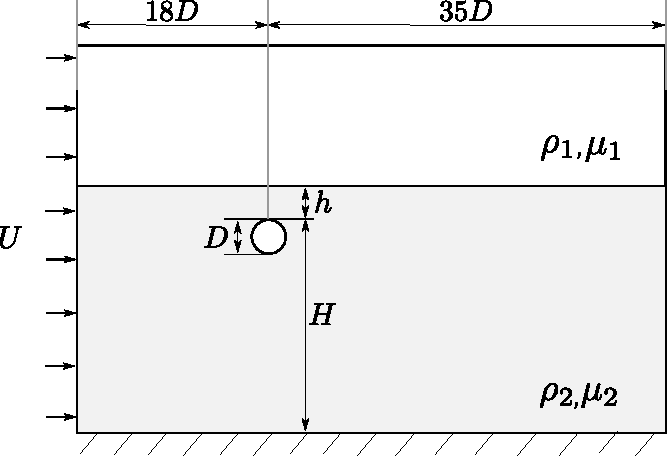
\includegraphics[width=.9\columnwidth]{config_2016.pdf}
    } \\
    %%----segunda subfigura----
%    \subfloat[Detailed Mesh]{
	  %\includegraphics[width=.9\columnwidth]{mesh_new.eps}
%%	  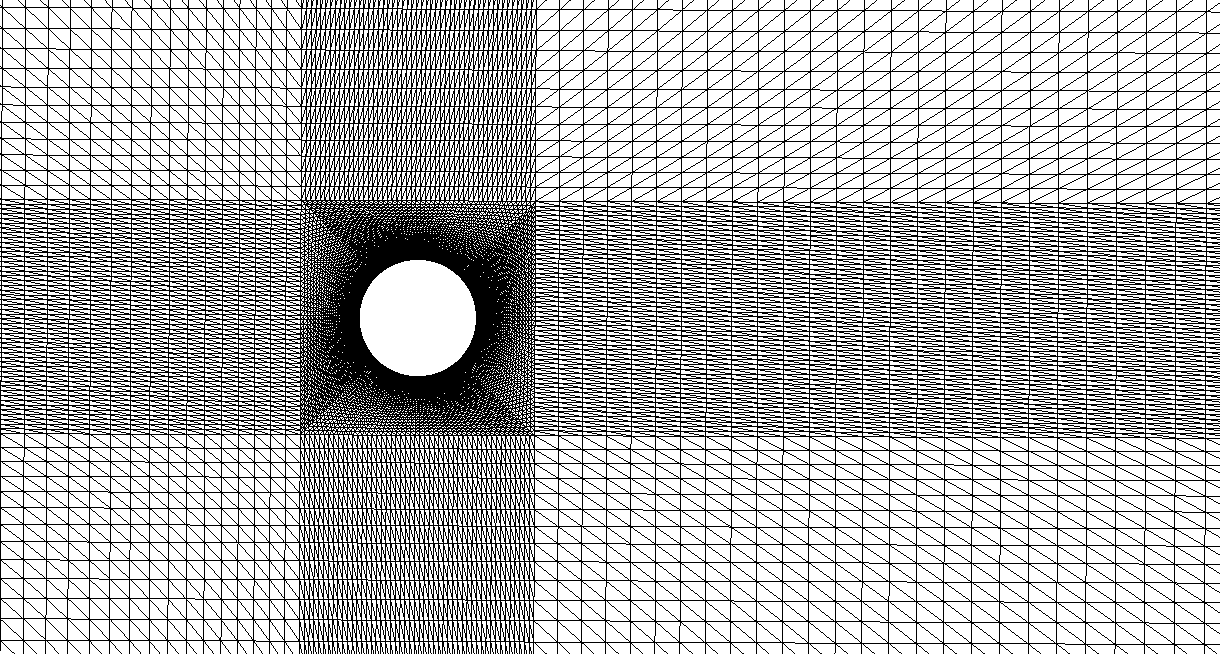
\includegraphics[width=.9\columnwidth]{mesh.png}
%    }
    \caption{General and detailed views of the mesh used for the baseflow computation and subsequent analysis, the circular cylinder is submerged a depth $h$.}
   \label{f:geometryandmesh}                %% Etiqueta para la figura entera
\end{figure}

An accurate and efficient simulation of the interface evolution is crucial in the simulation of free-surface flows. During the flow evolution, it is essential that the interface remains sharp. Large jumps of fluid density and viscosity across the interface should be correctly captured by the numerical algorithm in order to satisfy the momentum balance at the vicinity of the interface. Readers interested in more details of the PFEM-2 method and the enrichment technique used for the free surface definition may see \cite{Gimenez2015186}.

The complete analysis requires two steps: during the first one, the two-dimensional Navier-Stokes equations are solved for those $Re_D$ and $Fr_D$ values that finally reach a steady or periodic state $(\overline{\mathbf{v}}, \overline{p},\overline{\phi})$ known as base flow. For those cases where the Reynolds number is above the critical value and no steady state is obtained turning to a periodic case, a time averaged solution is analyzed, see \cite{SippLebedev} and the result will be confirmed by DMD analysis. During the second step, the base flow is perturbed by the product of a small parameter $\varepsilon\ll 1$ by the amplitude velocity $\widehat{\mathbf{v}}$ and kinematic pressure $\widehat{p}$ perturbations, as follows:

\begin{equation}
  \mathbf{v} = \overline{\mathbf{v}} + \varepsilon \widehat{\mathbf{v}}\exp(\omega t) \qquad p = \overline{p} + \varepsilon \widehat{p}\exp(\omega t)
\end{equation}

where the complex number $\omega=\omega_r+i\omega_i$ contains the growth rate as real part and the oscillation frequency as complex part. The stability analysis of the equations implies the linearization of the Navier-Stokes equations around a steady or mean base flow. This process has been done following the same methods explained in \cite{Gonzalez07} which implies the resolution of a large generalized eigenvalue problem by an iterative Arnoldi method. The baseflow can be considered unstable when any of the $\omega_r$ is positive. When the Navier-Stokes equations are solved and perturbed those gradients must be taken into account and new terms depending on the gradient of the kinematic viscosity are not negligible on the free surface proximities. However, two important considerations should be remarked when this analysis step is performed:

\begin{itemize}
 \item For subcritical Reynolds numbers, the steady baseflow implies a final distribution of both fluids determined by the values of the VOF function. As usual, the free surface is represented by the value 0 of the VOF function. The VOF function distribution is not perturbed for the analysis, assuming that the vortex shedding will be the cause of instability. This will be later confirmed by DMD analysis.
 \item For supercritical cases where the baseflow is unsteady, either a frequency damping algorithm or an averaged process is required to obtain a baseflow suitable for analysis \cite{jordi2015adaptive,SippLebedev}. In our case, the linear global stability analysis results using an averaged baseflow have been confirmed by a DMD analysis using no less than 10 snapshots per period.
\end{itemize}



%
% \begin{figure}
% \begin{center}
% \label{f:geometryandmesh}
%   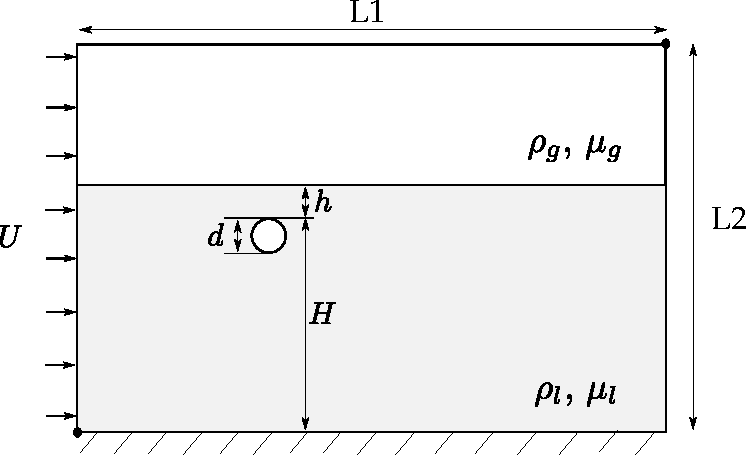
\includegraphics[width=.9\columnwidth]{config.pdf} \\
%
%   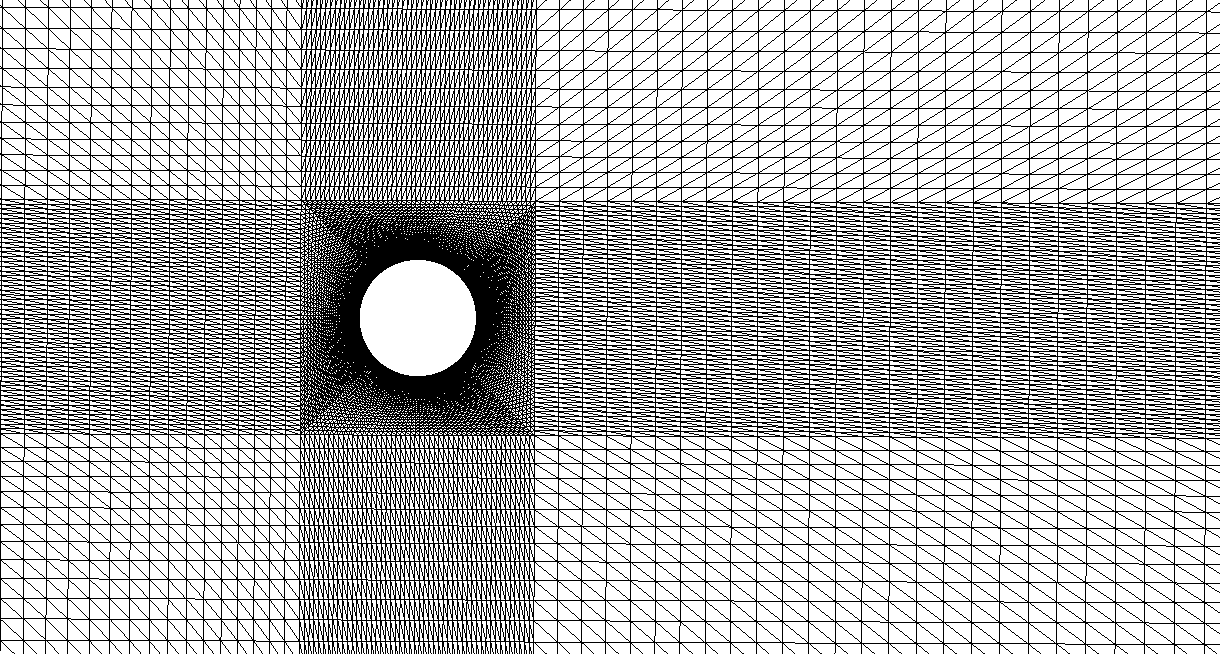
\includegraphics[width=.9\columnwidth]{mesh.png}
%   \end{center}
%   \caption{General and detailed views of the mesh used for the baseflow computation and subsequent analysis, the circular cylinder is submerged a depth $h$.}
% \end{figure}

%=====================================================================================
\section{Results}
\label{S:Results}
%=====================================================================================
For the case where the liquid (bottom fluid) density and fluid viscosity is 100 times their respective top fluid value, we have analyzed a range of Reynolds $Re=(30,70)$ in the proximities of $Re_C$. The Froude number has been kept fixed to $Fr_D=3$ and three different water depth values were studied $h/D=0.55,1,2$. Despite the Reynolds number difference, the free surface elevation at the top of the cylinder is similar to the one presented by Bouscasse \cite{Bouscasse14}. For the sake of code validation, the global drag and lift forces have been compared against previous results\cite{Bouscasse14} at the standard $Re_D=180, h/D=0.55$ and different Froude numbers being the agreement very satisfactory, see FIG. \ref{f:CdCl}.

\begin{figure}
  \begin{center}
  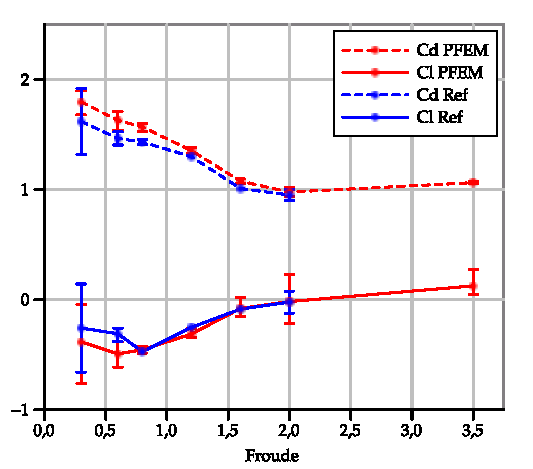
\includegraphics[width=6cm]{CdCl_Re180_hd_0_55.pdf}\\
  \end{center}
  \caption{Drag and Lift coefficients calculated with PFEM-2 at $Re_D=180$ and $h/D=0.55$ for different $Fr_D$ numbers, comparison with the reference work of Bouscasse \cite{Bouscasse14}.} \label{f:CdCl}
\end{figure}

\begin{figure}[ht]
  \centering
%    \subfloat[Horizontal velocity component from -0.15 (blue) to 2.15 (red)]{
%	  \label{uRe45}
	  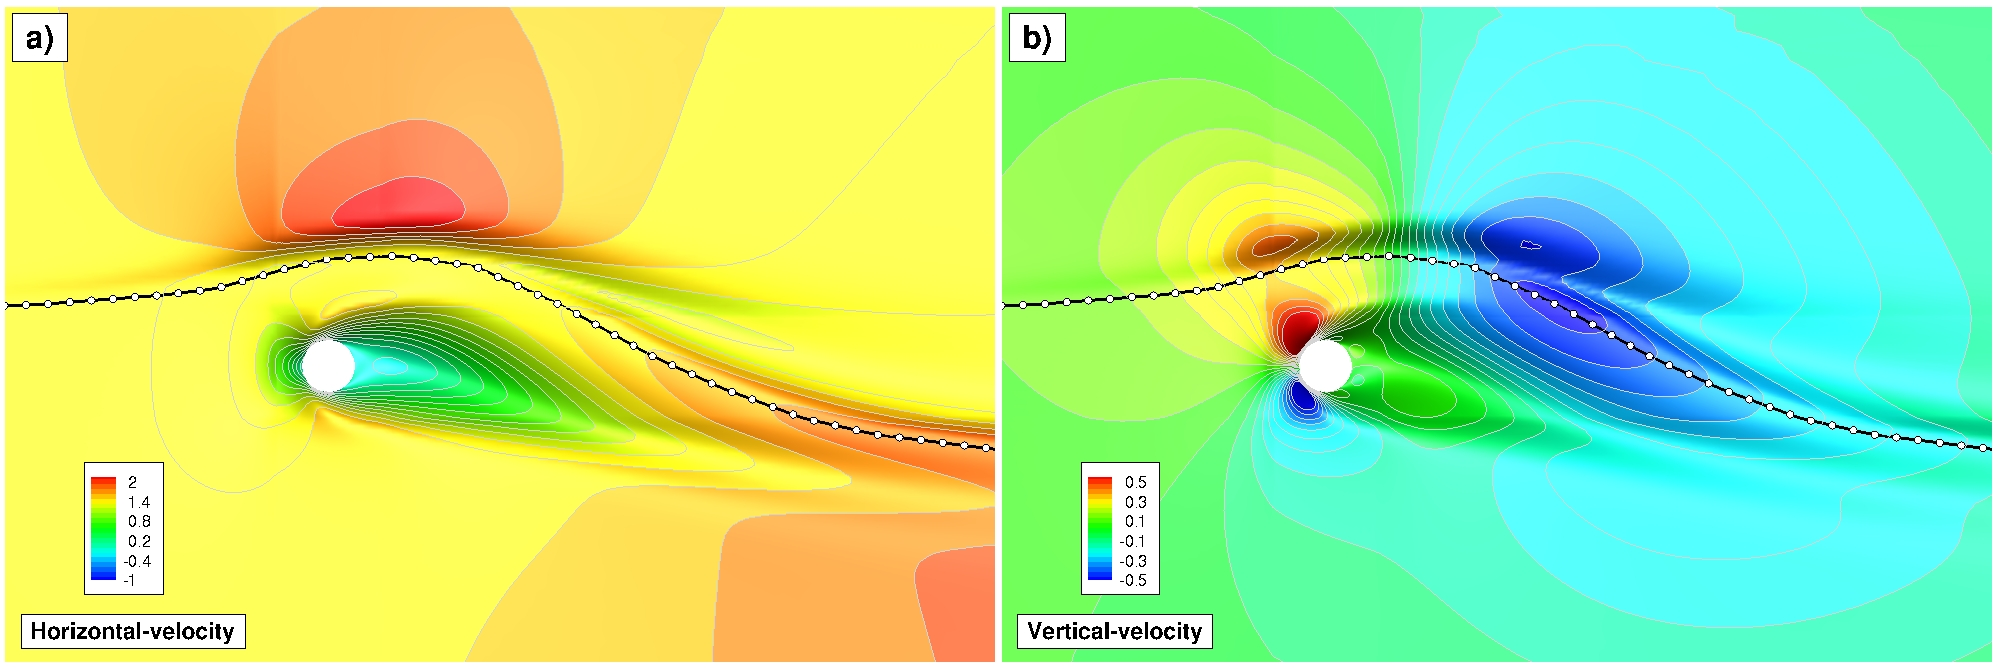
\includegraphics[width=1.1\columnwidth]{Leo_Base_flow_cyl.jpg}
    %}
    %\\
    %%----segunda subfigura----
%    \subfloat[Vertical velocity component from -0.65 (blue) to 0.75 (red)]{
%	  \label{vRe45}
%	  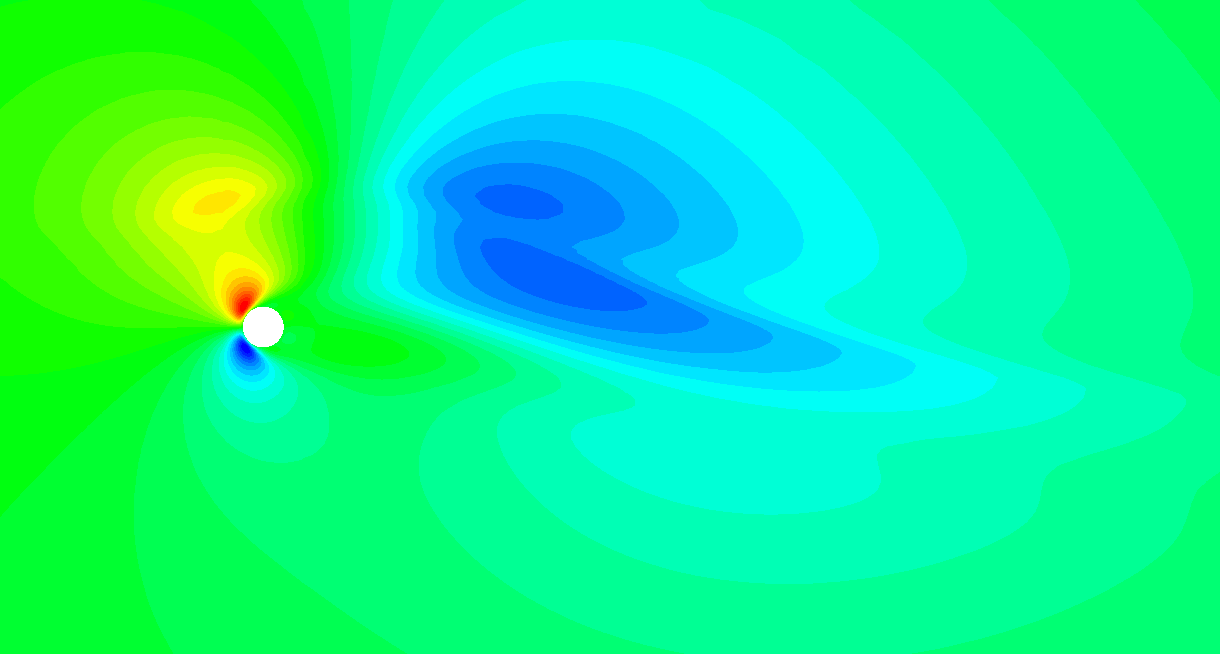
\includegraphics[width=.9\columnwidth]{vRe45.png}
%    } \\
    %\subfloat[To be removed]{
%	  \label{VOF}
%	  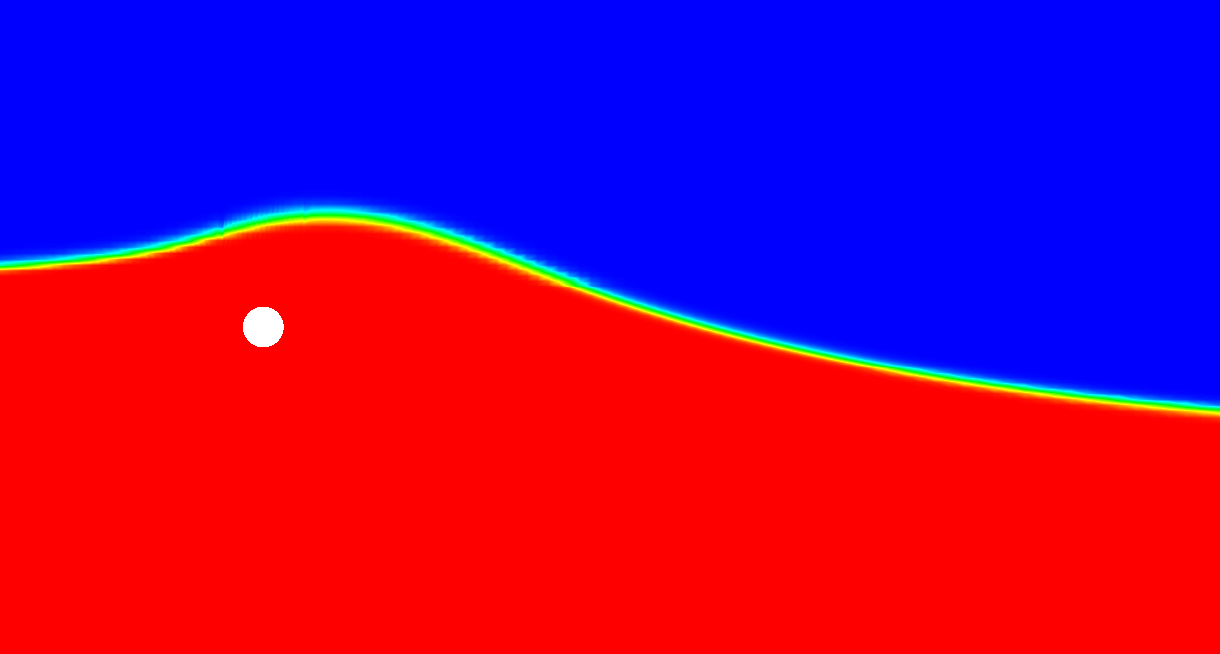
\includegraphics[width=.9\columnwidth]{vofRe45.png}
%    }
   \caption{Steady state solution for $Re_D=45$, $h/D=0.55$ and $Fr_D=3$}
   \label{f:baseflow}
\end{figure}

For the stability study, a collection of steady baseflows has been obtained varying the Reynolds number and the cylinder depth. As example, the horizontal and vertical velocity components of the baseflow and the free surface position corresponding to $Re_D=45$, $h/D=0.55$ and $Fr_D=3$ are shown in FIG. \ref{f:baseflow}. For each one a stability analysis based of the resolution of the large eigenvalue problem mentioned before has been computed, and the evolution of the most unstable mode monitored. The evolution of the growth/damping rate and the angular frequencies of the most unstable mode is shown in FIG. \ref{f:omegas}, where the value without free surface $h/D=\infty$ is also represented as reference. It can be observed that similarly to what happens in the absence of free surface and gravity the most unstable mode moves towards the unstable region $\omega_r<0$ when the Reynolds number is increased. For a Reynolds number very close to the one found in the absence of free surface and gravity $Re_c\approx 47$ the mode turns to be unstable and vortex shedding process develops. This critical value depends on the $h/D$ parameter, increasing when $h/D$ decreases. It is also worth noting that the free surface presence increases the stability of the flow. A black dot representing the less stable pure gravitational case without free surface ($h/D=\infty$) has been included in FIG. \ref{f:omegas} for comparison. An increasing oscillation is appreciated by the presence of the gravity field, being the critical frequencies for all cylinder depths noticeably higher that the one associated to the case without free surface and gravity $\omega_c=0.7414$. It can be hence concluded that both gravity and free surface affect the vortex shedding onset. A second fact is that the frequency associated to this oscillating unstable mode increases with the cylinder depth, having the case $h/D=2$ a frequency very close to the single phase case.

%This frequency can be confirmed when the global force is monitored while the Navier-Stokes equations are solved, see FIG. \ref{f:lifts}


\begin{figure}
  \begin{center}
    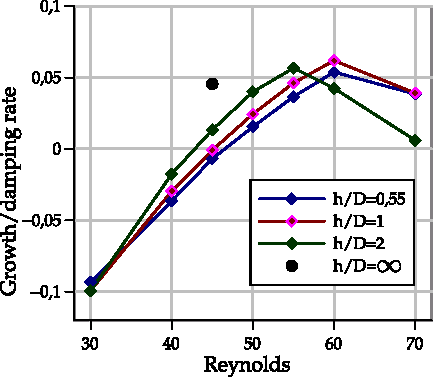
\includegraphics[width=5cm]{Growth_color.pdf}
    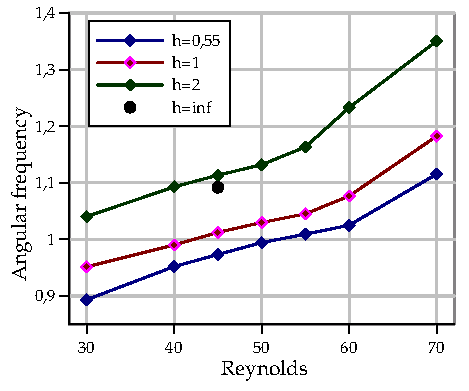
\includegraphics[width=5cm]{Freq_color.pdf}\\
  \end{center}
  \caption{Growth rate and frequency for different $Re$ numbers and $h/D$ values. The isolated black dot represents the case with gravity and without free surface ($h/D=\infty$). The classic result in the absence of free surface and gravity has $Re_c=47$ and $\omega_c=0.7414$ as critical values.}
  \label{f:omegas}
\end{figure}

In order to confirm if the averaged baseflows obtained for highest supercritical Reynolds values were correct, a DMD analysis has been performed for each cylinder depth. In FIG. \ref{f:freqDMD}, the critical frequencies from the most unstable mode DMD analysis are compared to the ones coming from the global analysis. As can be observed the values of the frequencies agree and the leading frequency was in all cases attributed to the vortex shedding phenomena aft the cylinder.

\begin{figure}
  \begin{center}
  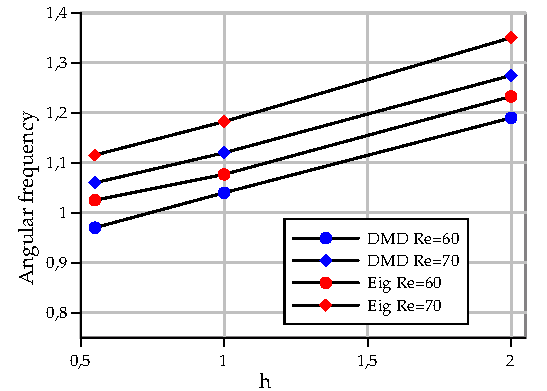
\includegraphics[width=0.7\columnwidth]{Freq_h_color.pdf}
  \end{center}
  \caption{Critical frequencies for different cylinder depths and Reynolds numbers are compared between DMD and global analysis.}
  \label{f:freqDMD}
\end{figure}

%\begin{figure}
%  \begin{center}
%  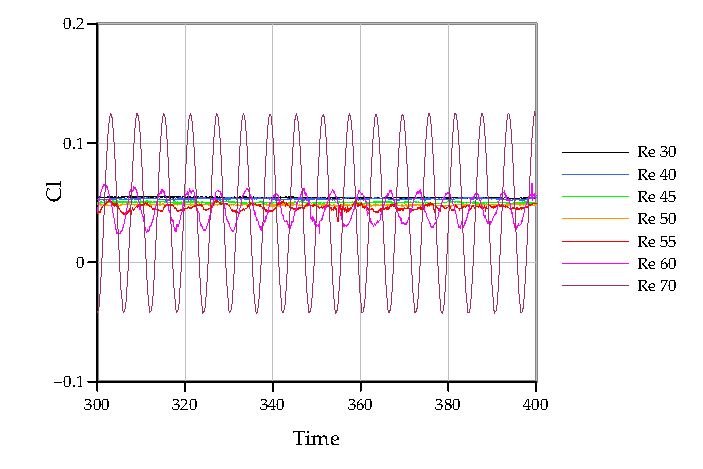
\includegraphics[width=\columnwidth]{Cl_Fr3_0.pdf}
%  \end{center}
%  \caption{Lift force at different Reynolds numbers.}
%  \label{f:lifts}
%\end{figure}

The mode corresponding to this oscillating unstable mode for the case $Re_D=45$ $Fr_D=3$ and $h/D=0.55$ is shown in FIG. \ref{f:mode}, where the shape of the mode is visibly influenced by the free surface modulation.

\begin{figure}[ht]
  \centering
  %  \subfloat[Horizontal velocity perturbation component (real part) from -0.1 (blue) to 0.1 (red)]{
%	  \label{pertuRe45}
	  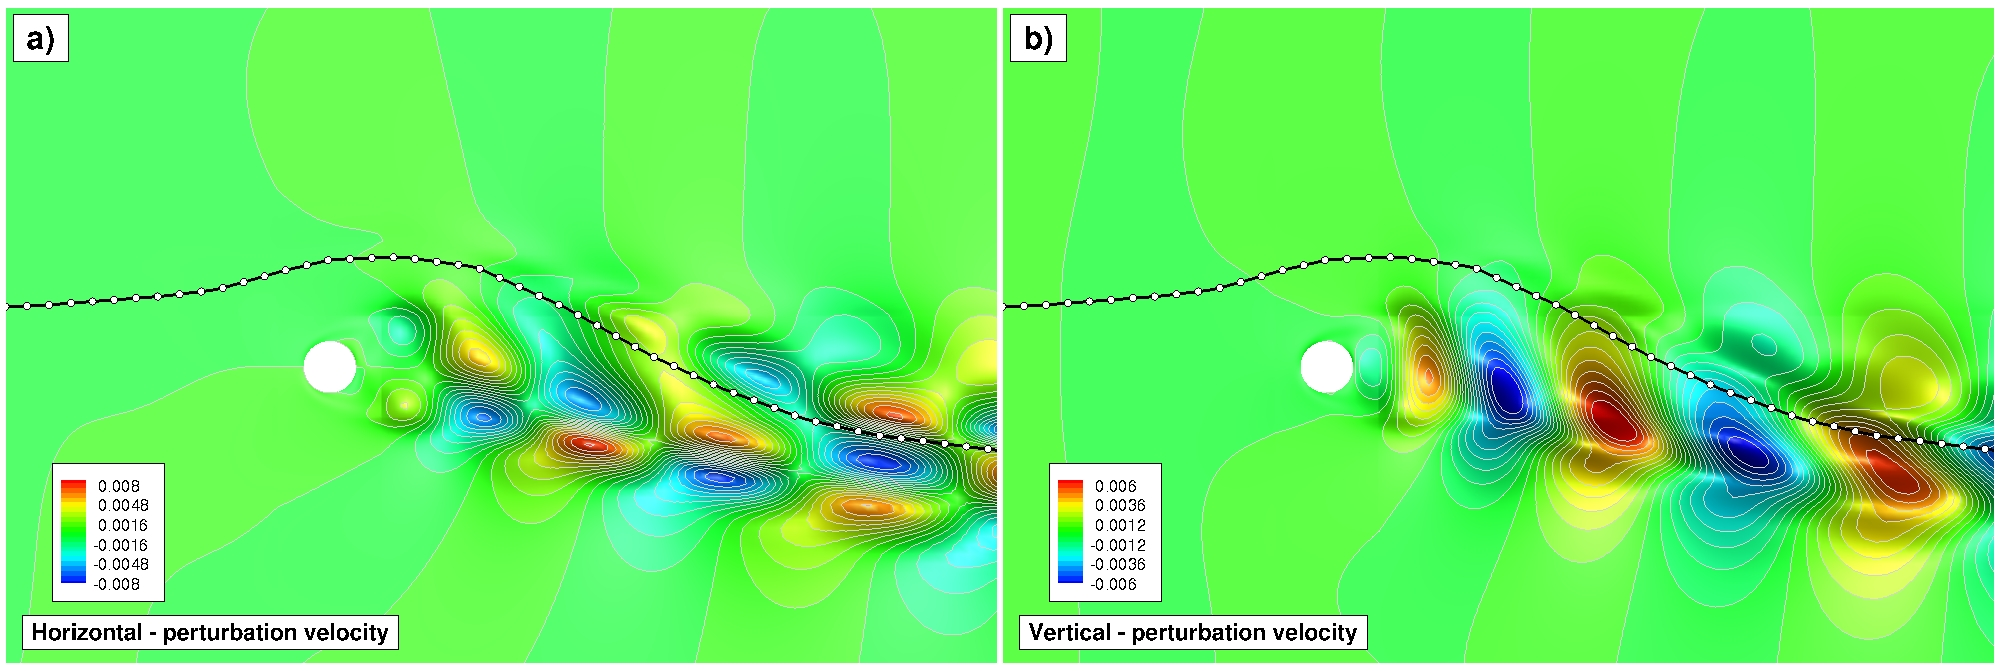
\includegraphics[width=.9\columnwidth]{Leo_Perturbation_cyl.jpg}
%    }
    %\\
    %%----segunda subfigura----
   % \subfloat[Vertical velocity perturbation component (real part) from -0.008 (blue) to 0.007 (red)]{
%	  \label{pertvRe45}
%	  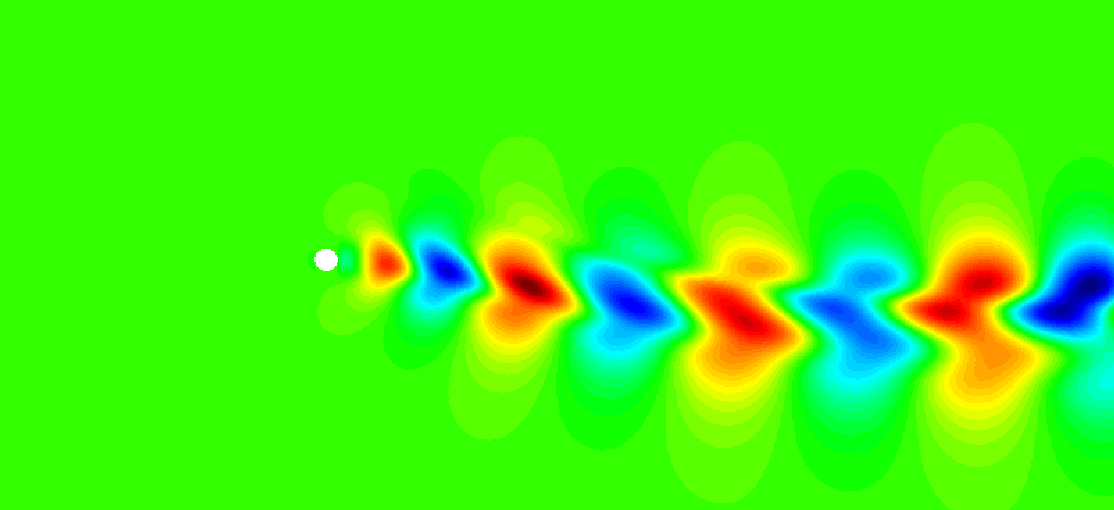
\includegraphics[width=.9\columnwidth]{pertvRe45.png}
%    }
  \caption{Unstable mode for the case $Re=45$ $Fr_D=3$ and $h/D=0.55$}
  \label{f:mode}
\end{figure}

% \begin{figure}
%   \begin{center}
%   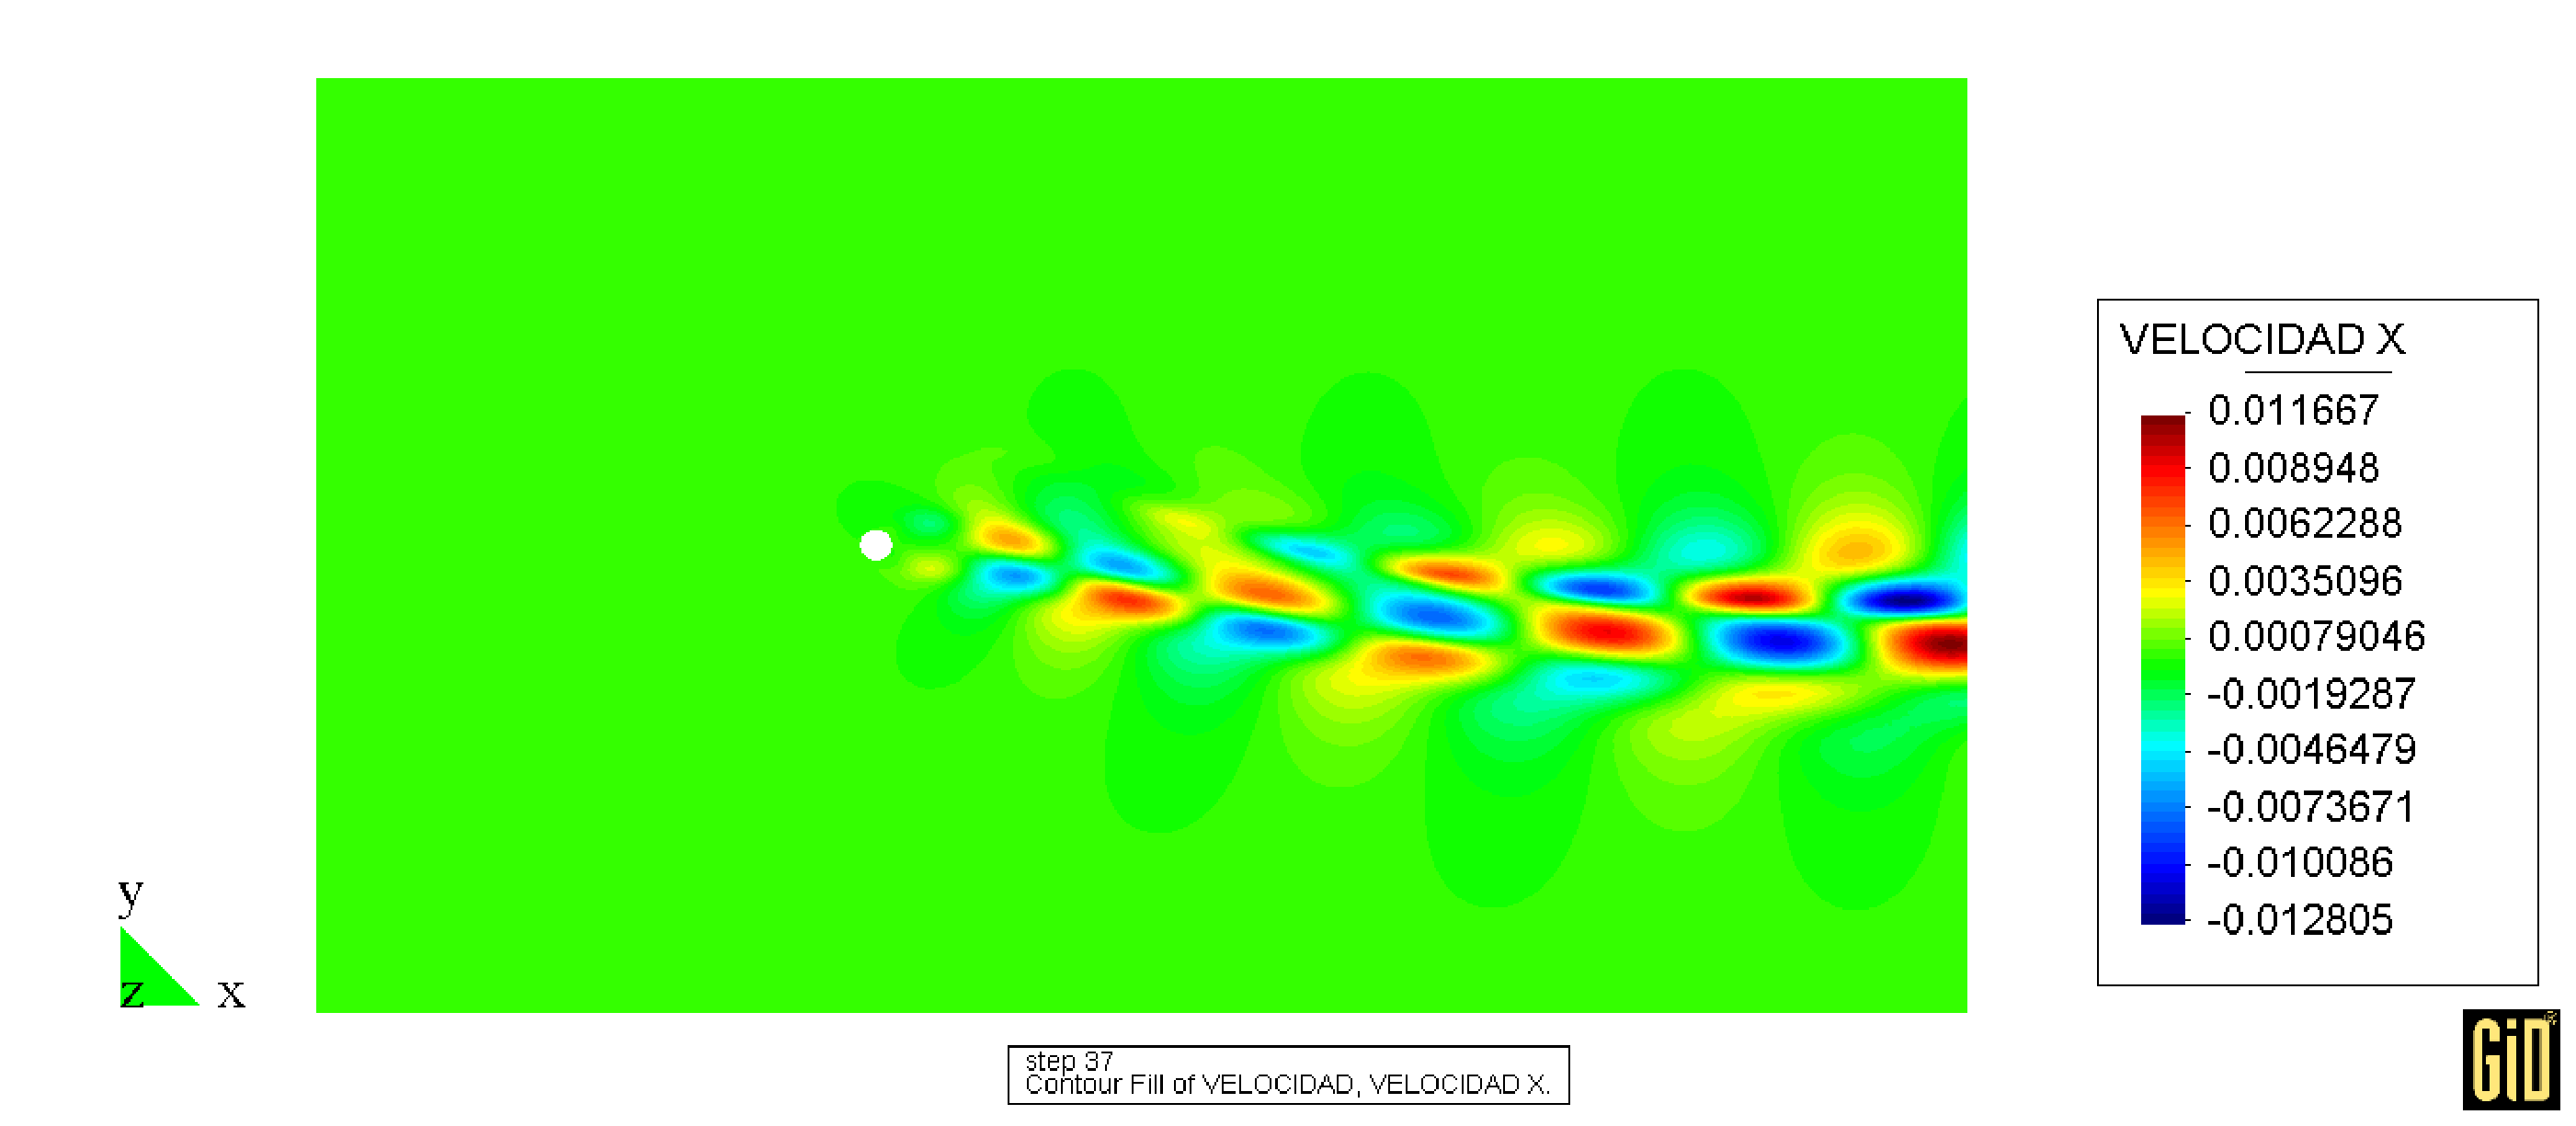
\includegraphics[width=6cm]{pertuRe45.eps}
%   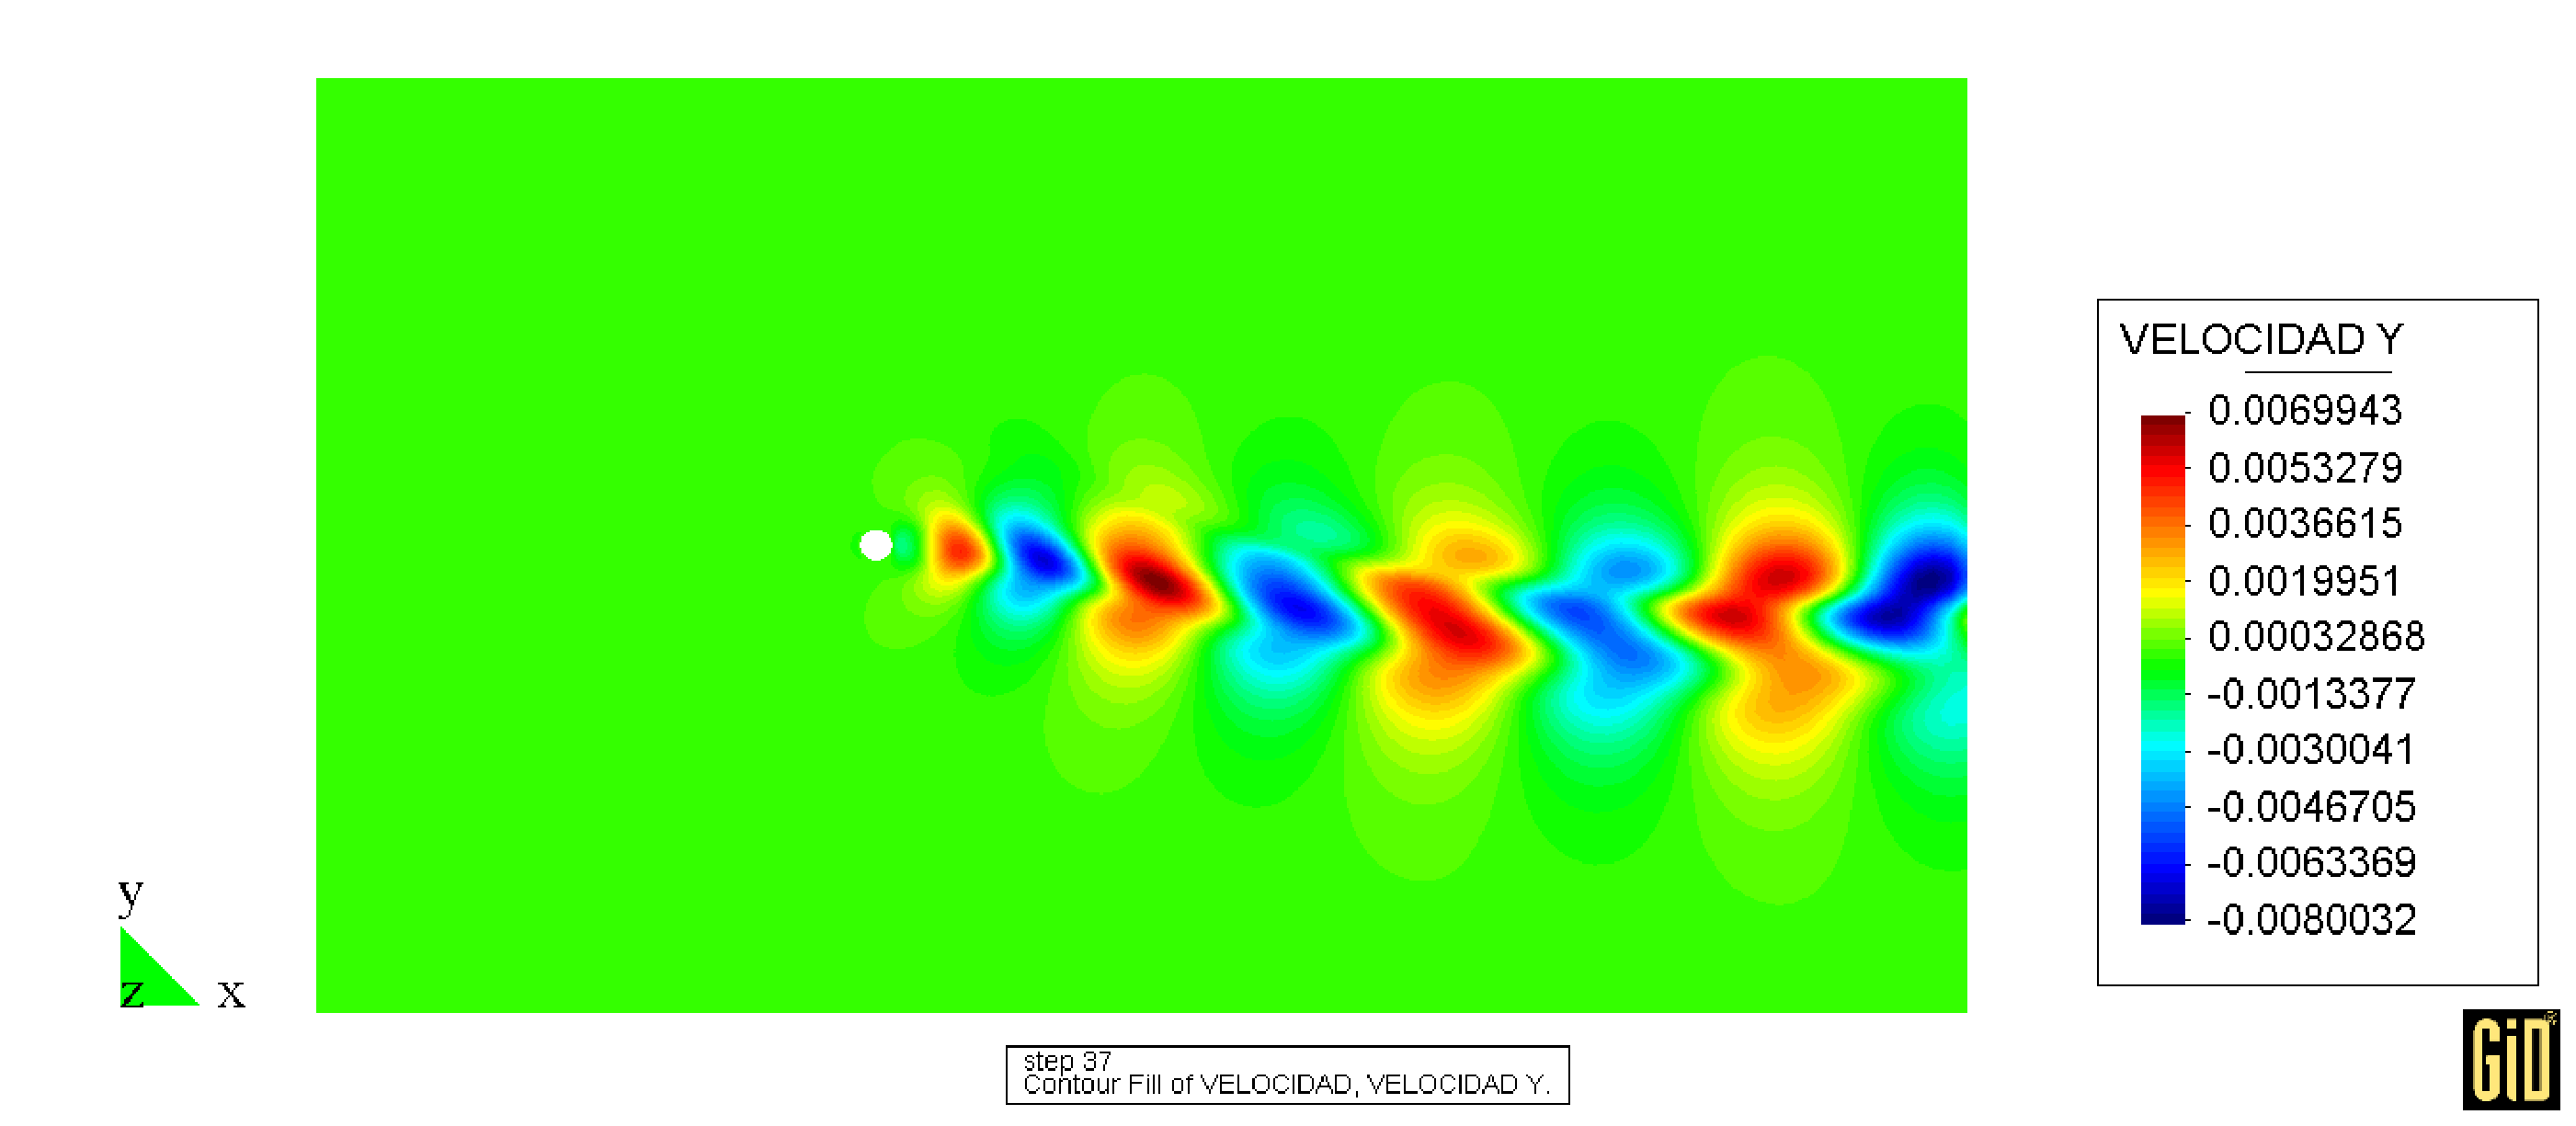
\includegraphics[width=6cm]{pertvRe45.eps}\\
%   \end{center}
%   \caption{Unstable mode $Re=45$ $Fr=3$}
%   \label{f:mode}
% \end{figure}

%According to Dimas results when the Froude number is above 2.5 as in our case the Branch II becomes dominant and instability becomes of the absolute type.\cite{Dimas89}

In the future these results will be also extended to higher Reynolds values by DMD analysis. Also the possibility of having situations such that growing instabilities caused by the free surface oscillations could also included in the analysis, similar to what occurs in a Rayleigh-Taylor instability. The possibility will be studied in future works. This work was supported by the Technical University of Madrid by the project (PID) "Combination of Eulerian and Lagrangian methodologies for the solution of free surface flows."


\bibliography{mybib}

\end{document}

% body of paper here - Use proper section commands
% References should be done using the \cite, \ref, and \label commands
\section{}
% Put \label in argument of \section for cross-referencing
%\section{\label{}}
\subsection{}
\subsubsection{}

% If in two-column mode, this environment will change to single-column
% format so that long equations can be displayed. Use
% sparingly.
%\begin{widetext}
% put long equation here
%\end{widetext}

% figures should be put into the text as floats.
% Use the graphics or graphicx packages (distributed with LaTeX2e)
% and the \includegraphics macro defined in those packages.
% See the LaTeX Graphics Companion by Michel Goosens, Sebastian Rahtz,
% and Frank Mittelbach for instance.
%
% Here is an example of the general form of a figure:
% Fill in the caption in the braces of the \caption{} command. Put the label
% that you will use with \ref{} command in the braces of the \label{} command.
% Use the figure* environment if the figure should span across the
% entire page. There is no need to do explicit centering.

% \begin{figure}
% \includegraphics{}%
% \caption{\label{}}
% \end{figure}

% Surround figure environment with turnpage environment for landscape
% figure
% \begin{turnpage}
% \begin{figure}
% \includegraphics{}%
% \caption{\label{}}
% \end{figure}
% \end{turnpage}

% tables should appear as floats within the text
%
% Here is an example of the general form of a table:
% Fill in the caption in the braces of the \caption{} command. Put the label
% that you will use with \ref{} command in the braces of the \label{} command.
% Insert the column specifiers (l, r, c, d, etc.) in the empty braces of the
% \begin{tabular}{} command.
% The ruledtabular enviroment adds doubled rules to table and sets a
% reasonable default table settings.
% Use the table* environment to get a full-width table in two-column
% Add \usepackage{longtable} and the longtable (or longtable*}
% environment for nicely formatted long tables. Or use the the [H]
% placement option to break a long table (with less control than
% in longtable).
% \begin{table}%[H] add [H] placement to break table across pages
% \caption{\label{}}
% \begin{ruledtabular}
% \begin{tabular}{}
% Lines of table here ending with \\
% \end{tabular}
% \end{ruledtabular}
% \end{table}

% Surround table environment with turnpage environment for landscape
% table
% \begin{turnpage}
% \begin{table}
% \caption{\label{}}
% \begin{ruledtabular}
% \begin{tabular}{}
% \end{tabular}
% \end{ruledtabular}
% \end{table}
% \end{turnpage}

% Specify following sections are appendices. Use \appendix* if there
% only one appendix.
%\appendix
%\section{}

% If you have acknowledgments, this puts in the proper section head.
%\begin{acknowledgments}
% put your acknowledgments here.
%\end{acknowledgments}

% Create the reference section using BibTeX:
\bibliography{basename of .bib file}

\end{document}
%
% ****** End of file apstemplate.tex ******

